% !TeX root = ../MAIN.tex
% !TeX encoding = UTF-8

\chapter{\LaTeX Beispiele}\label{chap2}

In diesem Beispiel werden einige Kommandos dieser Vorlage erklärt.

\section{Überschriften}\label{chap2_headings}

Es gibt unterschiedliche Ebenen von Überschriften. Diese können mit den Kommandos \verb|\section|, \verb|\subsection| und \verb|\subsubsection| erstellt werden. Versuchen Sie mehr als 3 Ebenen zu vermeiden!

\section{Dateien importieren}

Falls die Arbeit auf mehrere tex-Dateien aufgeteilt wird, können diese mit dem Kommando \verb|\input | importiert werden. Zum Beispiel: \verb|\input{introduction}|, dies importiert die Datei \texttt{introduction.tex}. \verb|% !TeX root = ../MAIN.tex
% !TeX encoding = UTF-8

\chapter{Einführung}
\label{chap:introduction}

Der inhaltliche Aufbau von Bachelor- bzw. Masterarbeiten, die am DKE-Institut durchgeführt werden, hat sich an folgender Aufzählung zu orientieren:

\begin{itemize}
	\item Kurzfassung (deutsch) bzw. Abstract (englisch)
	\item Einleitung mit Definition der Problemstellung (gemäß Exposé)
	\item Grundlagen / State-of-the-Art
	\item Beschreibung der Eigenleistung
	\item Fazit / Schlussfolgerungen
	\item (Anhang: ggf. Installationsanleitung, Benutzerhandbuch, etc.)
\end{itemize}

Die Beschreibung der Eigenleistung umfasst bei Implementierungsthemen folgende Punkte:

\begin{itemize}
	\item Anforderungen/Konzepte (Systemanalyse – WAS war zu implementieren?)
	\item Design bzw. Architektur der Software (Systembeschreibung/Spezifikation – WIE wurde das Geforderte umgesetzt?)
		\begin{itemize}
			\item Lösungsidee(n)
			\item Datenmodell der Software
			\item Komponenten / Module sowie deren interne und externe Abhängigkeiten
			\item Prozesse bzw. Abläufe von Algorithmen
		\end{itemize}
	\item Lösungsansatz, ggf. mit Darstellung unterschiedlicher Alternativen
	\item Schnittstelle der Software
	\item Test-/Erfahrungsbericht (z.B. Performancetests)
\end{itemize}

Die Beschreibung der Eigenleistung umfasst bei Literaturthemen folgende Punkte:

\begin{itemize}
	\item Vergleichskriterien (Kriterienkatalog, mit Motivation bzw. Begründung)
	\item Auswahl relevanter Literatur (mit Begründung)
	\item Analyse/Beschreibung der ausgewählten Ansätze in der relevanten Literatur
	\item Evaluierung der ausgewählten Ansätze anhand der Vergleichskriterien
\end{itemize}| importiert die Datei \texttt{chapter1.tex} aus dem Ordner \texttt{chapters}.

\subsection{Eine Subsektion}

\lipsum

\subsubsection{Eine Sub-Subsektion}

\lipsum

\section{Aufzählungen}\label{sec:enums}

Mit \verb|\itemize| können Listen erstellt werden; mit \verb|\enumerate| nummerierte Liste. Beide können mit den Kommandos \verb|\begin{itemize}| und \verb|\end{itemize}| bzw. \verb|\begin{enumerate}| und \verb|\end{enumerate}| erstellt werden.
 
Eine Ungeordnete Liste:
\begin{itemize}
  \item An Item
  \item Another Item
  \item Yet another Item
\end{itemize}

Eine nummerierte Liste:
\begin{enumerate}
  \item One
  \item Two
  \item Three
\end{enumerate}

\section{Zitierung}

Diese Vorlage verwendet BibLaTex mit Biber zur Verwaltung der Referenzen. Zitierungen können mit dem Kommando \verb|\cite| erfolgen. Zum Beispiel~\cite{PHD:Fielding}. Wahrscheinlich sind mehrere Durchläufe notwendig, bis alle Zitierungen und auch Referenzen korrekt dargestellt werden.

Andere Beispiele sind: \autocite{Gluchowski.2019} / \textcite{DBLP:conf/edbt/KovacicSSSS18} / \cite[S.~2]{DBLP:journals/ijcis/GolfarelliMR98}

\section{Referenzen}

Referenzen zu anderen Elementen, können mit \verb|\ref| erstellt werden. Die referenzierten Elemente müssen mit \verb|\label| gekennzeichnet werden.

Um zum Beispiel ein Kapitel, das mit \verb|\label{sec:enums}| gekennzeichnet wurde, zu referenzieren, muss \verb|\ref{sec:enums}| angegeben werden. Dies erzeugt die Nummer des Kapitels: ``In Kapitel~\ref{sec:enums}\ldots''.

Diese Vorlage beinhaltet ein paar benutzerdefinierte Kommandos, um das Referenzieren zu vereinfachen:

\begin{itemize}
    \item \verb|\citechap|:   ``In~\citechap{introduction} \ldots''
    \item \verb|\citesec|:    ``In~\citesec{enums} \ldots''
    \item \verb|\citefig|:    ``In~\citefig{sample-fig} \ldots''
    \item \verb|\citetable| : ``In~\citetable{example1} \ldots''
\end{itemize}

\section{Abbildungen}

Eine Abbildung kann mit \verb|\includegraphics| bzw. \verb|\includesvg| importiert werden, wie in \citefig{sample-fig} dargestellt.

\begin{figure}[ht!]
	\centering
	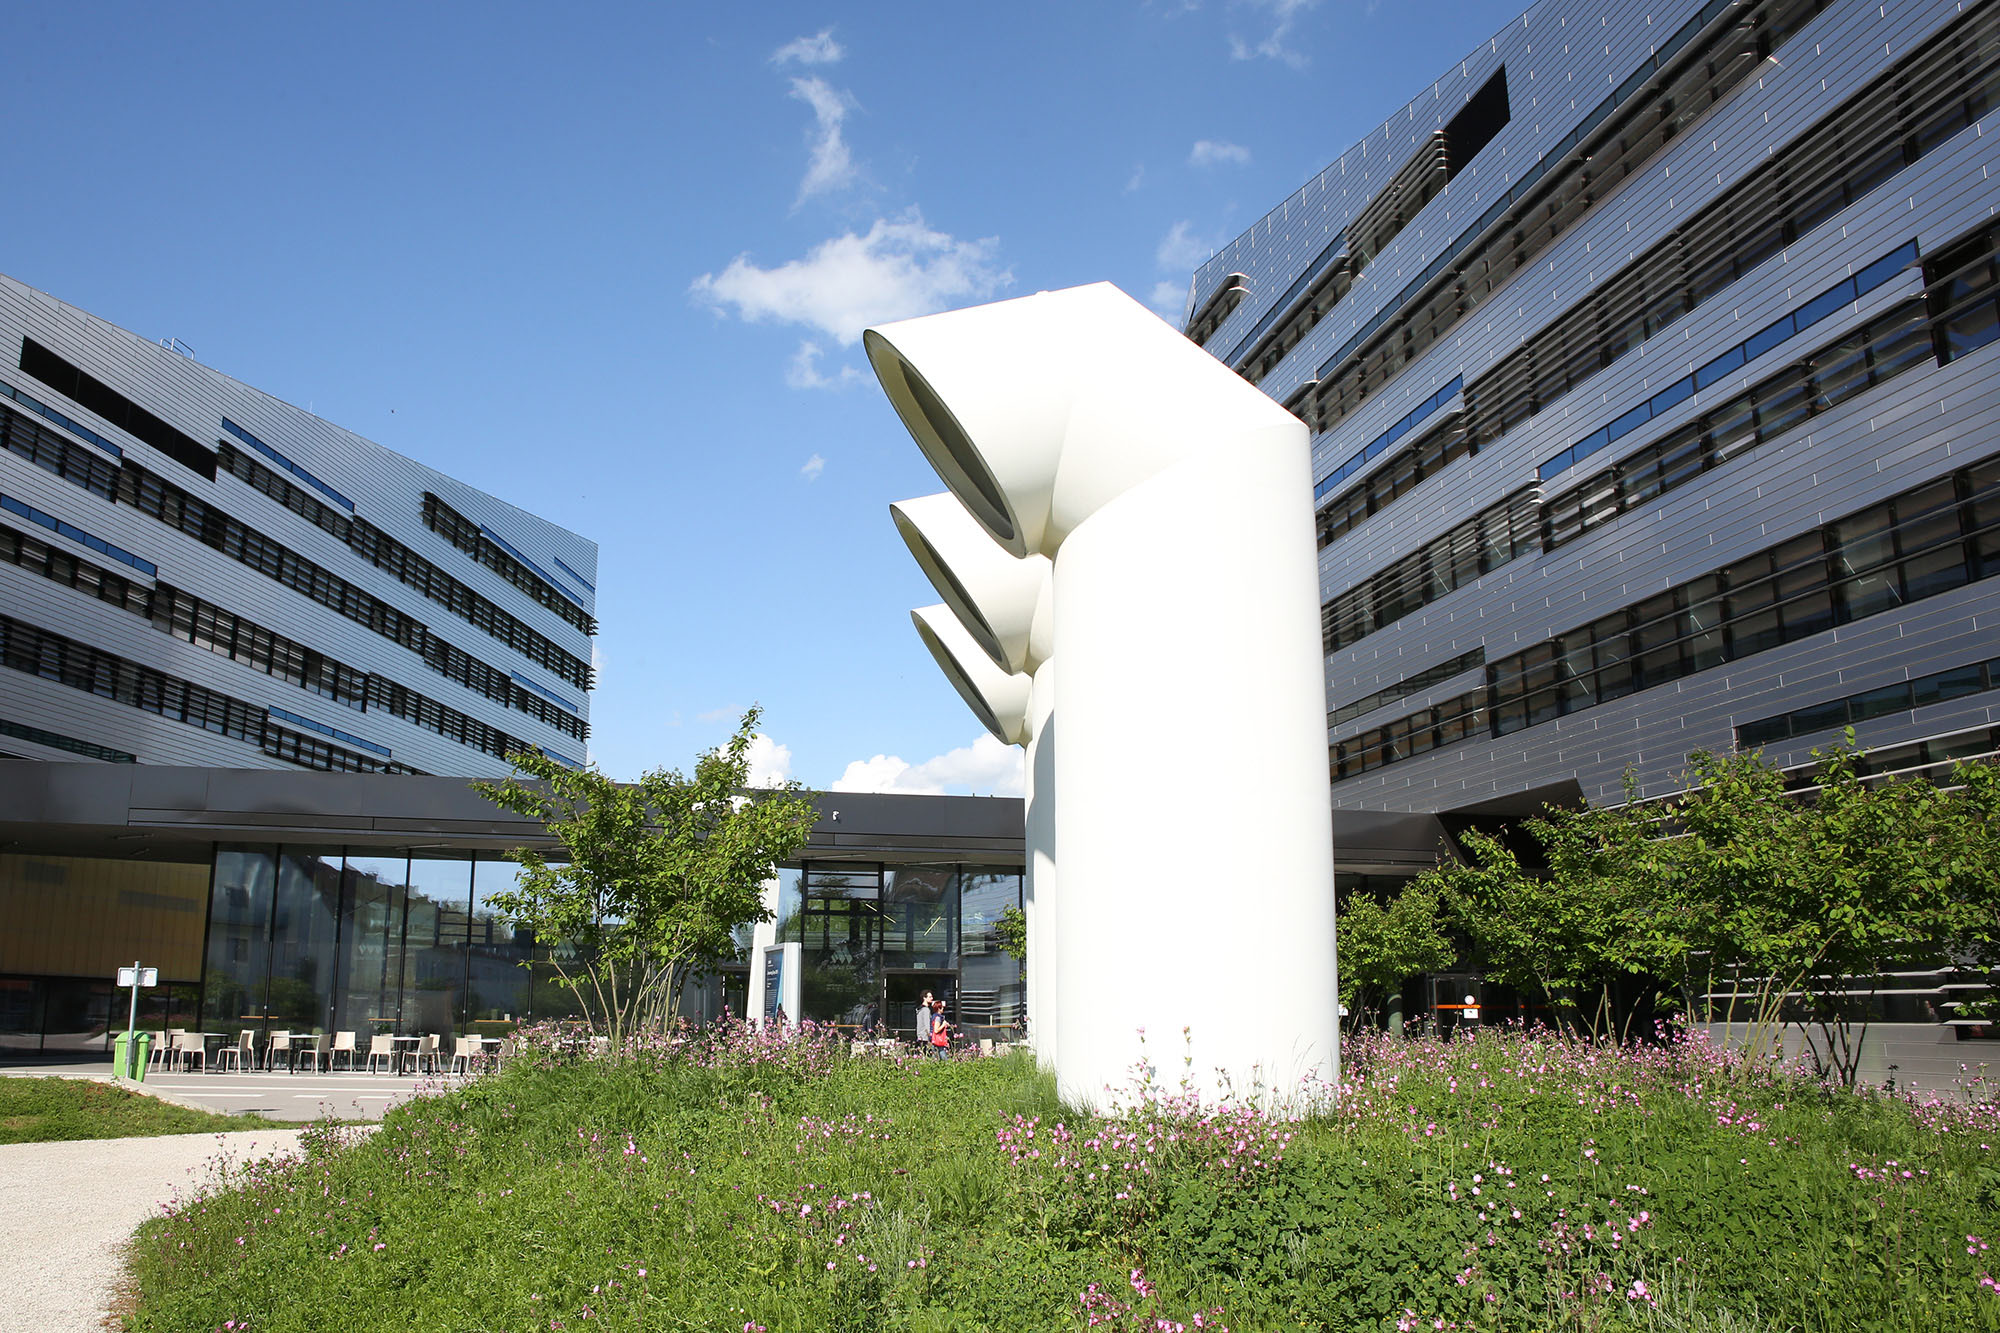
\includegraphics[width=0.4\linewidth]{figures/sciencepark.jpg}
	\caption{Ein Beispiel Bild (Johannes Kepler Universität)}
	\label{fig:sample-fig}
\end{figure}


\section{Tabellen}

Eine Tabelle kann in \LaTeX mit der \verb|tabular|-Umgebung oder einer Erweiterung davon (z.\thinspace{}B. \verb|tabularx|) erstellt werden. \citetable{example1} und \citetable{example2} zeigen Beispiel für Tabellen

\begin{table}[th!]
	\centering
	\caption{Beispiel einer Tabelle}\label{tab:example1}
	\begin{tabular}{p{4cm}r}
		\toprule
		Category                & Wind	Speed (Mph)             \\ \midrule
		1                       & 25                            \\
		2                       & 25                            \\
		3                       & 25                            \\ \midrule
		4                       & 25                            \\
		5                       & \textgreater{}=155           \\ \bottomrule
	\end{tabular}
\end{table}


\begin{table}[th!]
	\centering
	\caption{Beispiel einer anderen Tabelle}\label{tab:example2}
	\begin{tabularx}{\textwidth}{|H{0.4}|H{1.6}|}
		\hline
		Spalte 1	& Spalte 2 \\ \hline \hline
		Wert 1		& Wert 2   \\ \hline
		Wert 3		& Wert 4   \\ \hline
	\end{tabularx}
\end{table}